% Created 2021-12-25 Sat 16:39
\documentclass[9pt, b5paper]{article}
\usepackage[UTF8]{ctex}
\usepackage{xltxtra}
\usepackage{bera}
\usepackage[T1]{fontenc}
\usepackage[scaled]{beraserif}
\usepackage[scaled]{berasans}
\usepackage[scaled]{beramono}
\usepackage{graphicx}
\usepackage{xcolor}
\usepackage{multirow}
\usepackage{multicol}
\usepackage{float}
\usepackage{textcomp}
\usepackage{geometry}
\geometry{left=1.2cm,right=1.2cm,top=1.5cm,bottom=1.2cm}
\usepackage{algorithm}
\usepackage{algorithmic}
\usepackage{latexsym}
\usepackage{natbib}
\usepackage{minted}
\newminted{common-lisp}{fontsize=ootnotesize}
\usepackage[xetex,colorlinks=true,CJKbookmarks=true,linkcolor=blue,urlcolor=blue,menucolor=blue]{hyperref}
\author{deepwaterooo}
\date{\today}
\title{Kotlin Grammer}
\hypersetup{
  pdfkeywords={},
  pdfsubject={},
  pdfcreator={Emacs 27.1 (Org mode 8.2.7c)}}
\begin{document}

\maketitle
\tableofcontents


\section{空安全}
\label{sec-1}

\subsection{可空类型与非空类型}
\label{sec-1-1}
\begin{itemize}
\item Kotlin 的类型系统旨在消除来自代码空引用的危险,也称为《十亿美元的错误》。
\item 许多编程语言(包括 Java)中最常见的陷阱之一,就是访问空引用的成员会导致空引用异常。在 Java 中,这等同于 NullPointerException 或简称 NPE。
\item Kotlin 的类型系统旨在从我们的代码中消除 NullPointerException。NPE 的唯一可能的原因可能是:
\begin{itemize}
\item 显式调用 throw NullPointerException();
\item 使用了下文描述的 !! 操作符;
\item 有些数据在初始化时不一致,例如当:
\begin{itemize}
\item 传递一个在构造函数中出现的未初始化的 this 并用于其他地方(“泄漏 this”);
\item 超类的构造函数调用一个开放成员,该成员在派生中类的实现使用了未初始化的状态;
\end{itemize}
\item Java 互操作:
\begin{itemize}
\item 企图访问平台类型的 null 引用的成员;
\item 用于具有错误可空性的 Java 互操作的泛型类型,例如一段 Java 代码可能会向 Kotlin 的 MutableList<String> 中加入 null,这意味着应该使用 MutableList<String?> 来处理它;
\item 由外部 Java 代码引发的其他问题。
\end{itemize}
\end{itemize}
\item 在 Kotlin 中,类型系统区分一个引用可以容纳 null (可空引用)还是不能容纳(非空引用)。 例如,String 类型的常规变量不能容纳 null:
\end{itemize}
\begin{minted}[frame=lines,fontsize=\scriptsize,linenos=false]{kotlin}
var a: String = "ab"
var a: String = "abc" // 默认情况下,常规初始化意味着非空
a = null // 编译错误
\end{minted}
\begin{itemize}
\item 如果要允许为空,我们可以声明一个变量为可空字符串,写作 String?:
\end{itemize}
\begin{minted}[frame=lines,fontsize=\scriptsize,linenos=false]{kotlin}
var b: String? = "abc" // 可以设置为空
b = null // ok
print(b)
\end{minted}
\begin{itemize}
\item 现在,如果你调用 a 的方法或者访问它的属性,它保证不会导致 NPE,这样你就可以放心地使用:
\end{itemize}
\begin{minted}[frame=lines,fontsize=\scriptsize,linenos=false]{kotlin}
val l = a.length
\end{minted}
\begin{itemize}
\item 但是如果你想访问 b 的同一个属性,那么这是不安全的,并且编译器会报告一个错误:
\end{itemize}
\begin{minted}[frame=lines,fontsize=\scriptsize,linenos=false]{kotlin}
val l = b.length // 错误:变量“b”可能为空
\end{minted}
\begin{itemize}
\item 但是我们还是需要访问该属性,对吧?有几种方式可以做到。
\end{itemize}

\subsection{在条件中检测 null}
\label{sec-1-2}
\begin{itemize}
\item 首先,你可以显式检测 b 是否为 null,并分别处理两种可能:
\end{itemize}
\begin{minted}[frame=lines,fontsize=\scriptsize,linenos=false]{kotlin}
val l = if (b != null) b.length else -1
\end{minted}
\begin{itemize}
\item 编译器会跟踪所执行检测的信息,并允许你在 if 内部调用 length。 同时,也支持更复杂(更智能)的条件:
\end{itemize}
\begin{minted}[frame=lines,fontsize=\scriptsize,linenos=false]{kotlin}
val b: String? = "Kotlin"
if (b != null && b.length > 0) {
    print("String of length ${b.length}")
} else {
    print("Empty string")
}
// String of length 6
\end{minted}
\begin{itemize}
\item 请注意,这只适用于 b 是不可变的情况(即在检测和使用之间没有修改过的局部变量 ,或者不可覆盖并且有幕后字段的 val 成员),因为否则可能会发生在检测之后 b 又变为 null 的情。况
\end{itemize}

\subsection{安全的调用}
\label{sec-1-3}
\begin{itemize}
\item 你的第二个选择是安全调用操作符,写作 ?.:
\end{itemize}
\begin{minted}[frame=lines,fontsize=\scriptsize,linenos=false]{kotlin}
val a = "Kotlin"
val b: String? = null
println(b?.length)
println(a?.length) // 无需安全调用
\end{minted}
\begin{itemize}
\item 如果 b 非空,就返回 b.length,否则返回 null,这个表达式的类型是 Int?。
\item 安全调用在链式调用中很有用。例如,如果一个员工 Bob 可能会(或者不会)分配给一个部门, 并且可能有另外一个员工是该部门的负责人,那么获取 Bob 所在部门负责人(如果有的话)的名字,我们写作:
\end{itemize}
\begin{minted}[frame=lines,fontsize=\scriptsize,linenos=false]{kotlin}
bob?.department?.head?.name
\end{minted}
\begin{itemize}
\item 如果任意一个属性(环节)为空,这个链式调用就会返回 null。
\item 如果要只对非空值执行某个操作,安全调用操作符可以与 let 一起使用:
\end{itemize}
\begin{minted}[frame=lines,fontsize=\scriptsize,linenos=false]{kotlin}
val listWithNulls: List<String?> = listOf("Kotlin", null)
for (item in listWithNulls) {
    item?.let { println(it) } // 输出 Kotlin 并忽略 null
}
\end{minted}
\begin{itemize}
\item 安全调用也可以出现在赋值的左侧。这样,如果调用链中的任何一个接收者为空都会跳过赋值,而右侧的表达式根本不会求值:
\end{itemize}
\begin{minted}[frame=lines,fontsize=\scriptsize,linenos=false]{kotlin}
// 如果 `person` 或者 `person.department` 其中之一为空,都不会调用该函数:
person?.department?.head = managersPool.getManager()
\end{minted}

\subsection{Elvis 操作符}
\label{sec-1-4}
\begin{itemize}
\item 当我们有一个可空的引用 b 时,我们可以说“如果 b 非空,我使用它;否则使用某个非空的值”:
\end{itemize}
\begin{minted}[frame=lines,fontsize=\scriptsize,linenos=false]{kotlin}
val l: Int = if (b != null) b.length else -1
val l: Int = if (b != null) b.length else -1
\end{minted}
\begin{itemize}
\item 除了完整的 if-表达式,这还可以通过 Elvis 操作符表达,写作 ?::
\end{itemize}
\begin{minted}[frame=lines,fontsize=\scriptsize,linenos=false]{kotlin}
val l = b?.length ?: -1
val l = b?.length ?: -1
\end{minted}
\begin{itemize}
\item 如果 ?: 左侧表达式非空,elvis 操作符就返回其左侧表达式,否则返回右侧表达式。 请注意, \uline{当且仅当左侧为空时,才会对右侧表达式求值。}
\item 请注意, \uline{因为 throw 和 return 在 Kotlin 中都是表达式,所以它们也可以用在 elvis 操作符右侧。这可能会非常方便,例如,检测函数参数:}
\end{itemize}
\begin{minted}[frame=lines,fontsize=\scriptsize,linenos=false]{kotlin}
fun foo(node: Node): String? { // <<<==== 返回值可为空
    val parent = node.getParent() ?: return null
    val name = node.getName() ?: throw IllegalArgumentException("name expected")
    // ……
}
\end{minted}

\subsection{!! 操作符: 非空断言运算符(!!)}
\label{sec-1-5}
\begin{itemize}
\item 第三种选择是为 NPE 爱好者准备的:非空断言运算符(!!)将任何值转换为非空类型,若该值为空则抛出异常。我们可以写 b!! ,这会返回一个非空的 b 值 (例如:在我们例子中的 String)或者如果 b 为空,就会抛出一个 NPE 异常:
\end{itemize}
\begin{minted}[frame=lines,fontsize=\scriptsize,linenos=false]{kotlin}
val l = b!!.length
\end{minted}
\begin{itemize}
\item 因此,如果你想要一个 NPE,你可以得到它,但是你必须显式要求它,否则它不会不期而至。
\end{itemize}

\subsection{安全的类型转换}
\label{sec-1-6}
如果对象不是目标类型,那么常规类型转换可能会导致 ClassCastException。 另一个选择是使用安全的类型转换,如果尝试转换不成功则返回 null:
\begin{minted}[frame=lines,fontsize=\scriptsize,linenos=false]{kotlin}
val aInt: Int? = a as? Int
\end{minted}

\subsection{可空类型的集合}
\label{sec-1-7}
\begin{itemize}
\item 如果你有一个可空类型元素的集合,并且想要过滤非空元素,你可以使用 filterNotNull 来实现:
\end{itemize}
\begin{minted}[frame=lines,fontsize=\scriptsize,linenos=false]{kotlin}
val nullableList: List<Int?> = listOf(1, 2, null, 4)
val intList: List<Int> = nullableList.filterNotNull()
\end{minted}
\section{Kotlin中常量和静态方法}
\label{sec-2}
\subsection{常量}
\label{sec-2-1}
\subsubsection{Java中:}
\label{sec-2-1-1}
\begin{minted}[frame=lines,fontsize=\scriptsize,linenos=false]{java}
class StaticDemoActivity {
     public static final String LOAN_TYPE = "loanType";
     public static final String LOAN_TITLE = "loanTitle";
}
\end{minted}
\subsubsection{Kotlin中:}
\label{sec-2-1-2}
\begin{minted}[frame=lines,fontsize=\scriptsize,linenos=false]{java}
class StaticDemoActivity {
    companion object {
        val LOAN_TYPE = "loanType"
        val  LOAN_TITLE = "loanTitle"
    }
}
class StaticDemoActivity {
    companion object StaticParams{
        val  LOAN_TYPE = "loanType"
        val  LOAN_TITLE = "loanTitle"
    }
}
class StaticDemoActivity {
    companion object {
        const val LOAN_TYPE = "loanType"
        const val LOAN_TITLE = "loanTitle"
    }
}
\end{minted}
\begin{itemize}
\item 注:const 关键字用来修饰常量,且只能修饰 val,不能修饰var, companion object 的名字可以省略,可以使用 Companion来指代
\end{itemize}
\subsubsection{引用常量(这里的引用只针对于java引用kotlin代码)}
\label{sec-2-1-3}
\begin{itemize}
\item TestEntity类引用StaticDemoActivity中的常量
\end{itemize}
\begin{minted}[frame=lines,fontsize=\scriptsize,linenos=false]{java}
class TestEntity {
    public TestEntity () {
        String title = StaticDemoActivity.Companion.getLOAN_TITLE();
    }
}
class TestEntity {
    public TestEntity () {
        String title = StaticDemoActivity.StaticParams.getLOAN_TITLE();
    }
}
class TestEntity {
    public TestEntity () {
        String title = StaticDemoActivity.LOAN_TITLE;
        String type= StaticDemoActivity.LOAN_TYPE;
    }
}
\end{minted}
\subsection{静态方法}
\label{sec-2-2}
\begin{itemize}
\item Java代码:
\end{itemize}
\begin{minted}[frame=lines,fontsize=\scriptsize,linenos=false]{java}
class StaticDemoActivity {
    public static void test(){
    } 
}
\end{minted}
\begin{itemize}
\item Kotlin中:
\end{itemize}
\begin{minted}[frame=lines,fontsize=\scriptsize,linenos=false]{java}
    class StaticDemoActivity {
        companion object {
            fun test(){
            }
        }
    }
    class StaticDemoActivity {
        companion object StaticParams{
            fun test() {
            }    
        }
    }
\end{minted}
\subsubsection{引用静态方法(这里的引用只针对于java引用kotlin代码)}
\label{sec-2-2-1}
\begin{itemize}
\item TestEntity类引用StaticDemoActivity中的静态方法
\end{itemize}
\begin{minted}[frame=lines,fontsize=\scriptsize,linenos=false]{java}
class TestEntity {
    public TestEntity () {
        StaticDemoActivity.Companion.test();
    }
}
class TestEntity {
    public TestEntity () {
        StaticDemoActivity.StaticParams.test();
    }
}
\end{minted}
\begin{itemize}
\item companion object \{\}中用来修饰 静态常量,或者静态方法,单例等等
\end{itemize}

\section{Kotlin中的object 与companion object的区别}
\label{sec-3}
\begin{itemize}
\item 区别:
\begin{itemize}
\item companion object 类中只能一个 声明周期跟类同步,Only one companion object is allowed per class
\item objcet 没有限制声明  更多用在对象声明,对象表达式使用。
\begin{itemize}
\item 可以声明在类里  也可以声明在顶级包下 top-level declaration
\end{itemize}
\end{itemize}
\item 使用原则:       
\begin{itemize}
\item 如果想写工具类的功能,直接创建文件,写 top-level「顶层」函数。(声明在包下)
\item 如果需要继承别的类或者实现接口,就用 object 或 companion object。
\end{itemize}
\end{itemize}

\subsection{一、 object关键字}
\label{sec-3-1}
\begin{itemize}
\item object 关键字可以表达两种含义:一种是对象表达式,另一种是 对象声明。
\end{itemize}
\subsubsection{1、对象表达式}
\label{sec-3-1-1}
\begin{itemize}
\item 继承一个匿名对象
\end{itemize}
\begin{minted}[frame=lines,fontsize=\scriptsize,linenos=false]{java}
val textView = findViewById<TextView>(R.id.tv)
textView.setOnClickListener(object : OnClickListener {
        override fun onClick(p0: View?) {
            Toast.makeText(this@TestActivity, "点击事件生效", Toast.LENGTH_LONG)
        }
 
})
\end{minted}
\begin{itemize}
\item 上面代码其实就是我们经常要给 view 设置的点击事件,OnClickListener 事件是一个匿名类的对象,用object来修饰。
\end{itemize}
\subsubsection{2、对象声明}
\label{sec-3-1-2}
\begin{itemize}
\item 用object 修饰的类为静态类,里面的方法和变量都为静态的。
\end{itemize}
\begin{enumerate}
\item 2.1 直接声明类
\label{sec-3-1-2-1}
\begin{minted}[frame=lines,fontsize=\scriptsize,linenos=false]{java}
object DemoManager {
    private val TAG = "DemoManager"
    fun a() {
        Log.e(TAG,"此时 object 表示 声明静态内部类")
    }
}
\end{minted}
\item 2.2 声明静态内部类
\label{sec-3-1-2-2}
\begin{itemize}
\item 类内部的对象声明,没有被inner 修饰的内部类都是静态的
\end{itemize}
\begin{minted}[frame=lines,fontsize=\scriptsize,linenos=false]{java}
class DemoManager{
    object MyObject {
        fun a() {
            Log.e(TAG,"此时 object 表示 直接声明类")
        }
    }
}
\end{minted}
\begin{itemize}
\item 如果需要调用 a()方法
\item kotlin中调用
\end{itemize}
\begin{minted}[frame=lines,fontsize=\scriptsize,linenos=false]{java}
fun init() {
    MyObject.a()
}
\end{minted}
\begin{itemize}
\item java中调用
\end{itemize}
\begin{minted}[frame=lines,fontsize=\scriptsize,linenos=false]{java}
 MyObject.INSTANCE.a();
\end{minted}
\end{enumerate}

\subsection{二、companion object}
\label{sec-3-2}
\begin{itemize}
\item companion object 修饰为伴生对象,伴生对象在类中只能存在一个,类似于java中的静态方法 Java 中使用类访问静态成员,静态方法。
\end{itemize}
\begin{minted}[frame=lines,fontsize=\scriptsize,linenos=false]{java}
companion object {
    private val TAG = "DemoManager"
    fun b() {
        Log.e(TAG,"此时 companion objec t表示 伴生对象")
    }
}
\end{minted}
\begin{itemize}
\item kotlin 中调用
\end{itemize}
\begin{minted}[frame=lines,fontsize=\scriptsize,linenos=false]{java}
fun init(){
   b()
}
\end{minted}
\begin{itemize}
\item java 中调用
\end{itemize}
\begin{minted}[frame=lines,fontsize=\scriptsize,linenos=false]{java}
DemoManager.Companion.b();
\end{minted}
\begin{itemize}
\item companion object 相关的内容可以查阅 Kotlin中常量和静态方法 这篇文章,在这里不多在具体描述。
\end{itemize}
\subsection{三、在companion object中如何调用外部的成员变量}
\label{sec-3-3}
\subsubsection{3.1 为什么companion object 中调用不到外部成员变量}
\label{sec-3-3-1}
\begin{minted}[frame=lines,fontsize=\scriptsize,linenos=false]{java}
class DemoManager {
    private val MY_TAG = "DemoManager"
    fun init(){
       b()
    }
    companion object {
        fun b() {
            Log.e(MY_TAG,"此时 companion objec t表示 伴生对象")
        }
    }
}
\end{minted}
\begin{itemize}
\item 在上面代码中MY$_{\text{TAG}}$ 是不会被调用到的。
\item 原理很简单:
\item 在java中我们写一个静态方法,如果需要调用成员变量,是无法调用到的
\end{itemize}
\begin{minted}[frame=lines,fontsize=\scriptsize,linenos=false]{java}
private String TAG = "MainActivity";
public static void init(){
    Log.e(TAG,"init() ");
}
\end{minted}
\begin{itemize}
\item 只有将 TAG 修改为静态成员变量才能调用到
\end{itemize}
\begin{minted}[frame=lines,fontsize=\scriptsize,linenos=false]{java}
private static String TAG = "MainActivity";
public static void init(){
    Log.e(TAG,"init() ");
}
\end{minted}
\begin{itemize}
\item 由此可以看出来,java中静态方法调用成员变量,要求成员变量必须是静态的, 在kotlin 中也是一样,所以当companion object 中调用非静态的成员变量也是调用不到的。
\end{itemize}
\subsubsection{3.2 怎样解决才能调用到呢?}
\label{sec-3-3-2}
\begin{minted}[frame=lines,fontsize=\scriptsize,linenos=false]{java}
companion object {
    private val MY_TAG = "DemoManager"
    fun b() {
        Log.e(MY_TAG,"此时 companion objec t表示 伴生对象")
    }
}
\end{minted}
\begin{itemize}
\item 将所引用的成员变量也修饰静态的,这样就可以引用到了。
\item 再透彻一点,偏源码与反编译一点儿的: \url{https://www.cnblogs.com/webor2006/p/11210181.html}
\item \url{https://juejin.cn/post/6844903816446345224}
\end{itemize}

\section{伴生对象:  A few facts about Companion objects(写得比较深和透彻一点儿)}
\label{sec-4}
\begin{itemize}
\item Kotlin给Java开发者带来最大改变之一就是废弃了static修饰符。与Java不同的是在Kotlin的类中不允许你声明静态成员或方法。相反,你必须向类中添加Companion对象来包装这些静态引用: 差异看起来似乎很小,但是它有一些明显的不同。
\item 首先,companion伴生对象是个实际对象的单例实例。你实际上可以在你的类中声明一个单例,并且可以像companion伴生对象那样去使用它。这就意味着在实际开发中,你不仅仅只能使用一个静态对象来管理你所有的静态属性! companion这个关键字实际上只是一个快捷方式,允许你通过类名访问该对象的内容(如果伴生对象存在一个特定的类中,并且只是用到其中的方法或属性名称,那么伴生对象的类名可以省略不写)。就编译而言,下面的testCompanion()方法中的三行都是有效的语句。
\end{itemize}
\begin{minted}[frame=lines,fontsize=\scriptsize,linenos=false]{kotlin}
class TopLevelClass {
    companion object {
        fun doSomeStuff() {
        }
    }
    object FakeCompanion {
        fun doOtherStuff() {
        }
    }
}
fun testCompanion() {
    TopLevelClass.doSomeStuff()
    TopLevelClass.Companion.doSomeStuff()
    TopLevelClass.FakeCompanion.doOtherStuff()
}
\end{minted}
\begin{itemize}
\item 为了兼容的公平性,companion关键字还提供了更多选项,尤其是与Java互操作性相关选项。果您尝试在Java类中编写相同的测试代码,调用方式可能会略有不同:
\end{itemize}
\begin{minted}[frame=lines,fontsize=\scriptsize,linenos=false]{java}
public void testCompanion() {
    TopLevelClass.Companion.doSomeStuff();
    TopLevelClass.FakeCompanion.INSTANCE.doOtherStuff();
}
\end{minted}
\begin{itemize}
\item 区别在于: Companion作为Java代码中静态成员开放(实际上它是一个对象实例,但是由于它的名称是以大写的C开头,所以有点存在误导性),而FakeCompanion引用了我们的第二个单例对象的类名。在第二个方法调用中,我们需要使用它的INSTANCE属性来实际访问Java中的实例(你可以打开IntelliJ IDEA或AndroidStudio中的"Show Kotlin Bytecode"菜单栏,并点击里面"Decompile"按钮来查看反编译后对应的Java代码)
\item 在这两种情况下(不管是Kotlin还是Java),使用伴生对象Companion类比FakeCompanion类那种调用语法更加简短。此外,由于Kotlin提供一些注解,可以让编译器生成一些简短的调用方式,以便于在Java代码中依然可以像在Kotlin中那样简短形式调用。
\item @JvmField注解,例如告诉编译器不要生成getter和setter,而是生成Java中成员。在伴生对象的作用域内使用该注解标记某个成员,它产生的副作用是标记这个成员不在伴生对象内部作用域,而是作为一个Java最外层类的静态成员存在。从Kotlin的角度来看,这没有什么太大区别,但是如果你看一下反编译的字节代码,你就会注意到伴生对象以及他的成员都声明和最外层类的静态成员处于同一级别。
\item 另一个有用的注解 @JvmStatic.这个注解允许你调用伴生对象中声明的方法就像是调用外层的类的静态方法一样。但是需要注意的是:在这种情况下,方法不会和上面的成员一样移出伴生对象的内部作用域。因为编译器只是向外层类中添加一个额外的静态方法,然后在该方法内部又委托给伴生对象。
\item 一起来看一下这个简单的Kotlin类例子:
\end{itemize}
\begin{minted}[frame=lines,fontsize=\scriptsize,linenos=false]{kotlin}
class MyClass {
    companion object {
        @JvmStatic
        fun aStaticFunction() {}
    }
}
\end{minted}
\begin{itemize}
\item 这是相应编译后的Java简化版代码:
\end{itemize}
\begin{minted}[frame=lines,fontsize=\scriptsize,linenos=false]{java}
public class MyClass {
    public static final MyClass.Companion Companion = new MyClass.Companion();
    fun aStaticFunction() {//外层类中添加一个额外的静态方法
        Companion.aStaticFunction();//方法内部又委托给伴生对象的aStaticFunction方法
    }
    public static final class Companion {
         public final void aStaticFunction() {}
    }
}
\end{minted}
\begin{itemize}
\item 这里存在一个非常细微的差别,但在某些特殊的情况下可能会出问题。例如,考虑一下Dagger中的module(模块)。当定义一个Dagger模块时,你可以使用静态方法去提升性能,但是如果你选择这样做,如果您的模块包含静态方法以外的任何内容,则编译将失败。由于Kotlin在类中既包含静态方法,也保留了静态伴生对象,因此无法以这种方式编写仅仅包含静态方法的Kotlin类。
\item 但是不要那么快放弃! 这并不意味着你不能这样做,只是它需要一个稍微不同的处理方式:在这种特殊的情况下,你可以使用Kotlin单例(使用object对象表达式而不是class类)替换含有静态方法的Java类并在每个方法上使用@JvmStatic注解。如下例所示:在这种情况下,生成的字节代码不再显示任何伴生对象,静态方法会附加到类中。
\end{itemize}
\begin{minted}[frame=lines,fontsize=\scriptsize,linenos=false]{kotlin}
@Module
object MyModule {
    @Provides
    @Singleton
    @JvmStatic
    fun provideSomething(anObject: MyObject): MyInterface {
        return myObject
    }
}
\end{minted}
\begin{itemize}
\item 这又让你再一次明白了伴生对象仅仅是单例对象的一个特例。但它至少表明与许多人的认知是相反的,你不一定需要一个伴生对象来维护静态方法或静态变量。你甚至根本不需要一个对象来维护,只要考虑顶层函数或常量:它们将作为静态成员被包含在一个自动生成的类中(默认情况下,例如MyFileKt会作为MyFile.kt文件生成的类名,一般生成类名以Kt为后缀结尾)
\item 我们有点偏离这篇文章的主题了,所以让我们继续回到伴生对象上来。现在你已经了解了伴生对象实质就是对象,也应该意识到它开放了更多的可能性,例如继承和多态。
\item 这意味着你的伴生对象并不是没有类型或父类的匿名对象。它不仅可以拥有父类,而且它甚至可以实现接口以及含有对象名。它不需要被称为companion。这就是为什么你可以这样写一个Parcelable类:
\end{itemize}
\begin{minted}[frame=lines,fontsize=\scriptsize,linenos=false]{kotlin}
class ParcelableClass() : Parcelable {
    constructor(parcel: Parcel) : this()
    override fun writeToParcel(parcel: Parcel, flags: Int) {}
    override fun describeContents() = 0
    companion object CREATOR : Parcelable.Creator<ParcelableClass> {
        override fun createFromParcel(parcel: Parcel): ParcelableClass = ParcelableClass(parcel)
        override fun newArray(size: Int): Array<ParcelableClass?> = arrayOfNulls(size)
    }
}
\end{minted}
\begin{itemize}
\item 这里, 伴生对象名为CREATOR,它实现了Android中的Parcelable.Creator接口,允许遵守Parcelable约定,同时保持比使用@JvmField注释在伴随对象内添加Creator对象更直观。Kotlin中引入了@Parcelize注解,以便于可以获得所有样板代码,但是在这不是重点\ldots{}
\item 为了使它变得更简洁,如果你的伴生对象可以实现接口,它甚至可以使用Kotlin中的代理来执行此操作:
\end{itemize}
\begin{minted}[frame=lines,fontsize=\scriptsize,linenos=false]{kotlin}
class MyObject {
    companion object : Runnable by MyRunnable()
}
\end{minted}
\begin{itemize}
\item 这将允许您同时向多个对象中添加静态方法!请注意,伴生对象在这种情况下甚至不需要作用域体,因为它是由代理提供的。
\item 最后但同样重要的是,你可以为伴生对象定义扩展函数! 这就意味着你可以在现有的类中添加静态方法或静态属性,如下例所示:
\end{itemize}
\begin{minted}[frame=lines,fontsize=\scriptsize,linenos=false]{kotlin}
class MyObject {
    companion object
    fun useCompanionExtension() {
        someExtension()
    }
}
fun MyObject.Companion.someExtension() {}//定义扩展函数
\end{minted}
\begin{itemize}
\item 这样做有什么意义?我真的不知道。虽然Marcin Moskala建议使用此操作将静态工厂方法以Companion的扩展函数的形式添加到类中。
\item 总而言之,伴生对象不仅仅是为了给缺少static修饰符的使用场景提供解决方案:
\item 它们是真正的Kotlin对象,包括名称和类型,以及一些额外的功能。
\item 他们甚至可以不用于仅仅为了提供静态成员或方法场景。可以有更多其他选择,比如他们可以用作单例对象或替代顶层函数的功能。
\item 与大多数场景一样,Kotlin意味着在你设计过程需要有一点点转变,但与Java相比,它并没有真正限制你的选择。如果有的话,也会通过提供一些新的、更简洁的方式让你去使用它。
\item \url{https://cloud.tencent.com/developer/article/1381584} 这个某天上午的时候再读一遍就可以了
\item \url{http://www.4k8k.xyz/article/u013064109/89199478} 这个没读,扫一眼
\end{itemize}

\section{Kotlin-查看Kotlin编译成class后代码的三种方式}
\label{sec-5}
\subsection{在AndroidStudio中查看}
\label{sec-5-1}
\begin{itemize}
\item 第一步:选择你要查看你的kotlin文件,然后点击Tools-->Kotlin-->Show Kotlin Bytecode
\item 第二步:点击左上角的 Decompile 按钮就会弹出你想要的class源码
\end{itemize}
\subsection{方法二}
\label{sec-5-2}
\begin{itemize}
\item 利用命令行 javap [option] *.class 命令
\end{itemize}
\begin{center}
\begin{tabular}{ll}
\hline
子命令 & 输出信息\\
\hline
-l & 输出行和变量的表\\
-public & 只输出公共的方法和成员\\
-protected & 只输出public和protected类和成员\\
-package & 只输出包,public和protected类和成员,这是默认情况\\
-p -private & 输出所有类和成员\\
-s & 输出内部类型签名\\
-c & 对代码进行反汇编。 eg:类中每一个方法内,包含 java 字节码的指令\\
-verbose & 输出栈大小,方法参数的个数\\
-costants & 输出静态 final 常量\\
\hline
\end{tabular}
\end{center}
\begin{itemize}
\item 样码
\end{itemize}
\begin{minted}[frame=lines,fontsize=\scriptsize,linenos=false]{kotlin}
class TestMain {
    public val msg1 = "类中的变量"
    private val msg2 = "类中的变量"
    companion object {
        val msg3 = "伴生对象的变量"
    }
}
val msg4 = "Kotlin文件中的变量"
fun sayHello(msg: String) {
    println("msg=$msg")
}
fun main() {
    val msg5 = "我要看你的class文件"
    sayHello(msg5)
}
\end{minted}
\begin{itemize}
\item Javap -public 输出结果
\begin{itemize}
\item Javap -public     输出公共的方法和成员
\end{itemize}
\item 输出的结果为
\end{itemize}
\begin{minted}[frame=lines,fontsize=\scriptsize,linenos=false]{java}
// javap -public TestMainKt.class
// Compiled from "TestMain.kt"
public final class com.yobo.yobo_kotlin.TestMainKt {
  public static final java.lang.String getMsg2();
  public static final void sayHello(java.lang.String);
  public static final void main();
  public static void main(java.lang.String[]);
}
// javap -public TestMain.class
// Compiled from "TestMain.kt"
public final class com.yobo.yobo_kotlin.TestMain {
  public static final com.yobo.yobo_kotlin.TestMain$Companion Companion;
  public final java.lang.String getMsg1();
  public com.yobo.yobo_kotlin.TestMain();
  public static final java.lang.String access$getMsg3$cp();
}
\end{minted}
\begin{itemize}
\item javap -p -private 
\begin{itemize}
\item javap -p -private  显示所有的类和成员
\end{itemize}
\item javap -p -private  TestMainKt.class
\end{itemize}
\begin{minted}[frame=lines,fontsize=\scriptsize,linenos=false]{java}
public final class com.yobo.yobo_kotlin.TestMainKt {
  private static final java.lang.String msg4;
  public static final java.lang.String getMsg4();
  public static final void sayHello(java.lang.String);
  public static final void main();
  public static void main(java.lang.String[]);
  static {};
}
\end{minted}
\begin{itemize}
\item Javap -c 输出结果
\begin{itemize}
\item Javap -c    对代码进行反汇编。 eg:类中每一个方法内,包含 java 字节码的
\end{itemize}
\item 可以看到虽然是把我们整个class文件进行了反编译,但是可读性不是很好,这时候我们就推荐第二种方法。
\end{itemize}
\begin{minted}[frame=lines,fontsize=\scriptsize,linenos=false]{java}
public final class com.yobo.yobo_kotlin.TestMainKt {
  public static final java.lang.String getMsg2();
    Code:
       0: getstatic     #13                 // Field msg2:Ljava/lang/String;
       3: areturn

  public static final void sayHello(java.lang.String);
    Code:
       0: aload_0
       1: ldc           #17                 // String msg
       3: invokestatic  #23                 // Method kotlin/jvm/internal/Intrinsics.checkParameterIsNotNull:(Ljava/lang/Object;Ljava/lang/String;)V
       6: new           #25                 // class java/lang/StringBuilder
       9: dup
      10: invokespecial #29                 // Method java/lang/StringBuilder."<init>":()V
      13: ldc           #31                 // String msg=
      15: invokevirtual #35                 // Method java/lang/StringBuilder.append:(Ljava/lang/String;)Ljava/lang/StringBuilder;
      18: aload_0
      19: invokevirtual #35                 // Method java/lang/StringBuilder.append:(Ljava/lang/String;)Ljava/lang/StringBuilder;
      22: invokevirtual #38                 // Method java/lang/StringBuilder.toString:()Ljava/lang/String;
      25: astore_1
      26: iconst_0
      27: istore_2
      28: getstatic     #44                 // Field java/lang/System.out:Ljava/io/PrintStream;
      31: aload_1
      32: invokevirtual #50                 // Method java/io/PrintStream.println:(Ljava/lang/Object;)V
      35: return
 
  public static final void main();
    Code:
       0: ldc           #56                 // String 我要看你的class文件
       2: astore_0
       3: aload_0
       4: invokestatic  #58                 // Method sayHello:(Ljava/lang/String;)V
       7: return
 
  public static void main(java.lang.String[]);
    Code:
       0: invokestatic  #54                 // Method main:()V
       3: return
 
  static {};
    Code:
       0: ldc           #8                  // String Kotlin文件中的变量
       2: putstatic     #13                 // Field msg2:Ljava/lang/String;
       5: return
}
\end{minted}
\subsection{Jadx反编译工具}
\label{sec-5-3}
\begin{itemize}
\item 先给出工具的GitHub地址,可以按照自己喜欢的方式安装并查看功能文档:
\begin{itemize}
\item \url{https://github.com/skylot/jadx}
\end{itemize}
\end{itemize}

\section{Synchronized、Volatile}
\label{sec-6}
\subsection{如何创建线程 Thread}
\label{sec-6-1}
在Kotlin 中,我们仍然可以使用 java 的语法创建一个线程
\begin{minted}[frame=lines,fontsize=\scriptsize,linenos=false]{kotlin}
Thread(Runnable { 
}).start()
// 或者使用 Lambda 表达式
Thread {
}.start()
\end{minted}
事实上,kotlin 为我们提供了一个简单写法:
Kotlin中可以使用thread()方法创建新的线程,指定的语句块将在新线程中运行。语法简单,十分易用。
\begin{minted}[frame=lines,fontsize=\scriptsize,linenos=false]{kotlin}
fun main() {
    thread {
        Log.d("yanjun", "开启一个线程")
    }
}
\end{minted}
用法够简单吧。你会好奇thread \{\}到底是什么黑科技,其实很简单,语法糖而已。 其实是一个 thread() \{\} 函数
\begin{minted}[frame=lines,fontsize=\scriptsize,linenos=false]{kotlin}
public fun thread(start: Boolean = true,
                  isDaemon: Boolean = false,
                  contextClassLoader: ClassLoader? = null,
                  name: String? = null,
                  priority: Int = -1,
                  block: () -> Unit
): Thread {
    val thread = object : Thread() {
        public override fun run() {
            block()
        }
    }
    if (isDaemon) thread.isDaemon = true
    if (priority > 0) thread.priority = priority
    if (name != null) thread.name = name
    if (contextClassLoader != null) thread.contextClassLoader = contextClassLoader
    if (start) thread.start()   
    return thread
}
\end{minted}
\begin{itemize}
\item 可以看到 start 参数默认为 true ,自动执行线程。当然也可以通过 name 字段指定线程的名字:
\end{itemize}
\begin{minted}[frame=lines,fontsize=\scriptsize,linenos=false]{kotlin}
fun main() {
    //指定线程的名字,是否自动执行
    thread(start = true, name = "my_thread") {
    }
}
\end{minted}
\subsection{如何使用 Synchronized 同步锁}
\label{sec-6-2}
\begin{itemize}
\item 在Java中,给一个方法加锁 ,需要给方法加 synchronized 关键字
\end{itemize}
\begin{minted}[frame=lines,fontsize=\scriptsize,linenos=false]{java}
public synchronized void run() {
}
\end{minted}
\begin{itemize}
\item kotlin 中没有 synchronized 关键之,取而代之的是 @Synchronized 注解
\end{itemize}
\begin{minted}[frame=lines,fontsize=\scriptsize,linenos=false]{kotlin}
class Util {
    @Synchronized
    fun main() {
    }
}
\end{minted}
\begin{itemize}
\item 我们把 kotlin 代码反编译一下看看,
\end{itemize}
\begin{minted}[frame=lines,fontsize=\scriptsize,linenos=false]{java}
public final class Util {
    public final synchronized void main() {
    }
}
\end{minted}
\begin{itemize}
\item 可以看到 @Synchronized 注解 可以达到 Java synchronized 关键字的作用。
\item 除此之外,kotlin 在方法内,可以使用 block 块
\end{itemize}
\subsubsection{例子1}
\label{sec-6-2-1}
\begin{minted}[frame=lines,fontsize=\scriptsize,linenos=false]{kotlin}
class Util {
    val lock = Any()
    fun main() {
        synchronized(this) {
        }
    }
}
\end{minted}
\begin{itemize}
\item 编译成 java 如下
\begin{minted}[frame=lines,fontsize=\scriptsize,linenos=false]{java}
public static final class Util {
    @NotNull
        private final Object lock = new Object();
    @NotNull
        public final Object getLock() {
        return this.lock;
    }
    public final void main() {
        synchronized(this) {
            boolean var2 = false;
            Unit var4 = Unit.INSTANCE;
        }
    }
}
\end{minted}
\end{itemize}
\subsubsection{例子2}
\label{sec-6-2-2}
\begin{minted}[frame=lines,fontsize=\scriptsize,linenos=false]{kotlin}
class Util {
    val lock = Any()
    fun main() {
        synchronized(lock) {
        }
    }
}
\end{minted}
\begin{itemize}
\item 编译成 java 如下
\begin{minted}[frame=lines,fontsize=\scriptsize,linenos=false]{java}
public static final class Util {
    @NotNull
        private final Object lock = new Object();
    @NotNull
        public final Object getLock() {
        return this.lock;
    }
    public final void main() {
        Object var1 = this.lock;
        synchronized(var1) {
            boolean var2 = false;
            Unit var4 = Unit.INSTANCE;
        }
    }
}
\end{minted}
\end{itemize}
\subsection{Volatile 关键字}
\label{sec-6-3}
\begin{itemize}
\item 在kotlin中没有volatile关键字,但是有 @Volatile 注解
\end{itemize}
\begin{minted}[frame=lines,fontsize=\scriptsize,linenos=false]{kotlin}
class Util {
    @Volatile
    var lock = Any()
}
\end{minted}
\begin{itemize}
\item 编译成 java 如下
\begin{minted}[frame=lines,fontsize=\scriptsize,linenos=false]{java}
public static final class Util {
    @NotNull
        private volatile Object lock = new Object();
    @NotNull
        public final Object getLock() {
        return this.lock;
    }
    public final void setLock(@NotNull Object var1) {
        Intrinsics.checkNotNullParameter(var1, "<set-?>");
        this.lock = var1;
    }
}
\end{minted}
\end{itemize}

\subsection{默认赋值}
\label{sec-6-4}
\subsubsection{默认不为空}
\label{sec-6-4-1}
\begin{minted}[frame=lines,fontsize=\scriptsize,linenos=false]{kotlin}
class A(val name: String, val age: Int)
\end{minted}
\begin{itemize}
\item 代表 name、age 不能为 null , 转换成 java , 会看到在构造函数中会对 name 字段做 空校验。
\begin{minted}[frame=lines,fontsize=\scriptsize,linenos=false]{java}
public static final class A {
    @NotNull
        private final String name;
    private final int age;
    @NotNull
        public final String getName() {
        return this.name;
    }
    public final int getAge() {
        return this.age;
    }
    public A(@NotNull String name, int age) {
        Intrinsics.checkNotNullParameter(name, "name");
        super();
        this.name = name;
        this.age = age;
    }
}
\end{minted}
\item 函数 checkNotNullParameter()源码如下:
\end{itemize}

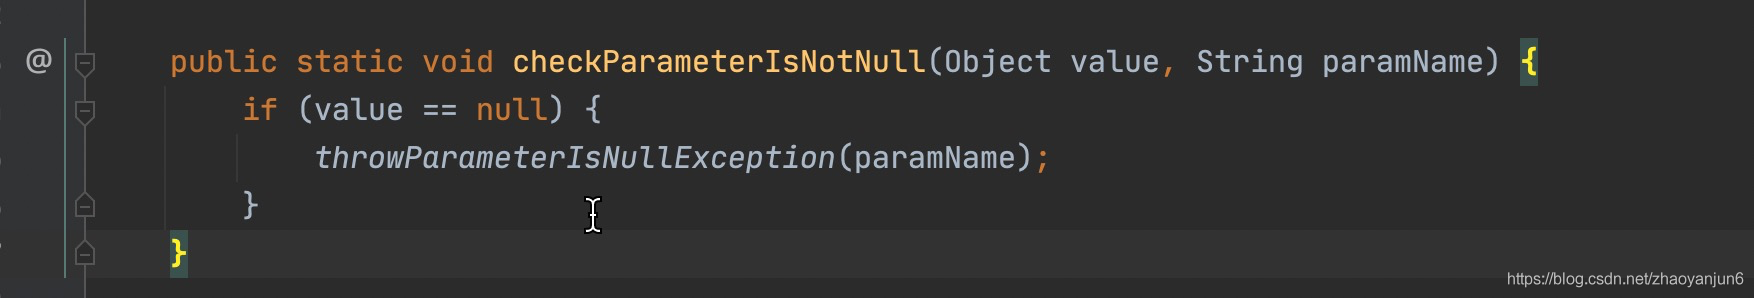
\includegraphics[width=.9\linewidth]{./pic/eg5.png}

\subsubsection{可以为空}
\label{sec-6-4-2}
\begin{minted}[frame=lines,fontsize=\scriptsize,linenos=false]{kotlin}
class A(val name: String?, val age: Int)
\end{minted}
\begin{itemize}
\item 代表 name 可为 null , 转换成 java , 会看到在构造函数中没有对 name 字段做 空校验。
\begin{minted}[frame=lines,fontsize=\scriptsize,linenos=false]{java}
public static final class A {
    @Nullable
        private final String name;
    private final int age;
    @Nullable
        public final String getName() {
        return this.name;
    }
    public final int getAge() {
        return this.age;
    }
    public A(@Nullable String name, int age) {
        this.name = name;
        this.age = age;
    }
}
\end{minted}
\end{itemize}

\subsubsection{默认值}
\label{sec-6-4-3}
\begin{minted}[frame=lines,fontsize=\scriptsize,linenos=false]{kotlin}
class A(val name: String? = "zhaoyanjun", val age: Int)
\end{minted}
\begin{itemize}
\item name 可为空,如果name 为null, 使用默认值 “zhaoyanjun”
\begin{minted}[frame=lines,fontsize=\scriptsize,linenos=false]{java}
public static final class A {
    @Nullable
        private final String name;
    private final int age;
    @Nullable
        public final String getName() {
        return this.name;
    }
    public final int getAge() {
        return this.age;
    }
    public A(@Nullable String name, int age) {
        this.name = name;
        this.age = age;
    }
    // $FF: synthetic method
    public A(String var1, int var2, int var3, DefaultConstructorMarker var4) {
        if ((var3 & 1) != 0) {
            var1 = "zhaoyanjun";
        }
        this(var1, var2);
    }
}
\end{minted}
\end{itemize}

\subsubsection{两个默认值}
\label{sec-6-4-4}
\begin{minted}[frame=lines,fontsize=\scriptsize,linenos=false]{kotlin}
class A(val name: String? = "zhaoyanjun", val age: Int ?= 10)
\end{minted}
\begin{itemize}
\item 出来的java码:
\begin{minted}[frame=lines,fontsize=\scriptsize,linenos=false]{java}
public static final class A {
    @Nullable
        private final String name;
    @Nullable
        private final Integer age;
    @Nullable
        public final String getName() {
        return this.name;
    }
    @Nullable
        public final Integer getAge() {
        return this.age;
    }
    public A(@Nullable String name, @Nullable Integer age) {
        this.name = name;
        this.age = age;
    }
    // $FF: synthetic method
    public A(String var1, Integer var2, int var3, DefaultConstructorMarker var4) {
        if ((var3 & 1) != 0) 
            var1 = "zhaoyanjun";
        if ((var3 & 2) != 0) 
            var2 = 10;
        this(var1, var2);
    }
}
\end{minted}
\end{itemize}

\subsection{构造函数}
\label{sec-6-5}
\begin{minted}[frame=lines,fontsize=\scriptsize,linenos=false]{kotlin}
class A(val name: String, val age: Int)
var a1 =  A("zhaoyanjun",10)  //编译正常
var a =  A()  //编译失败,因为没有无参构造函数
\end{minted}
\begin{minted}[frame=lines,fontsize=\scriptsize,linenos=false]{java}
public static final class A {
    @NotNull
        private final String name;
    private final int age;
    @NotNull
        public final String getName() {
        return this.name;
    }
    public final int getAge() {
        return this.age;
    }
    public A(@NotNull String name, int age) {
        Intrinsics.checkNotNullParameter(name, "name");
        super();
        this.name = name;
        this.age = age;
    }
}
\end{minted}
\begin{itemize}
\item 如何才能调用无参构造函数呢?其实很简单,给每个参数添加一个默认值就可以了
\end{itemize}
\begin{minted}[frame=lines,fontsize=\scriptsize,linenos=false]{kotlin}
class A(val name: String? = "", val age: Int? = 0)
\end{minted}
\begin{itemize}
\item 只要参数都有默认值,就会默认生成 无参构造函数
\begin{minted}[frame=lines,fontsize=\scriptsize,linenos=false]{java}
public static final class A {
    @Nullable
        private final String name;
    @Nullable
        private final Integer age;
    @Nullable
        public final String getName() {
        return this.name;
    }
    @Nullable
        public final Integer getAge() {
        return this.age;
    }
    public A(@Nullable String name, @Nullable Integer age) {
        this.name = name;
        this.age = age;
    }
    // $FF: synthetic method
    public A(String var1, Integer var2, int var3, DefaultConstructorMarker var4) {
        if ((var3 & 1) != 0) 
            var1 = "";
        if ((var3 & 2) != 0) 
            var2 = 0;
        this(var1, var2);
    }
}
\end{minted}
\end{itemize}

\subsection{重载函数 @JvmOverloads}
\label{sec-6-6}
\begin{minted}[frame=lines,fontsize=\scriptsize,linenos=false]{kotlin}
class A(val name: String, val age: Int)
var a1 =  A("zhaoyanjun",10)   //编译正常
var a2 =  A("123")    //编译失败,没有只有一个参数的构造函数
\end{minted}
\begin{itemize}
\item 如何才能自动生成重载函数呢?其实很简单
\item 给每个参数添加默认值
\item 标记 constructor 关键字
\item 标记 @JvmOverloads 关键字
\end{itemize}
\begin{minted}[frame=lines,fontsize=\scriptsize,linenos=false]{kotlin}
class A @JvmOverloads constructor(val name: String? = "", val age: Int? = 0)
\end{minted}
\begin{itemize}
\item 生成的java码如下:
\begin{minted}[frame=lines,fontsize=\scriptsize,linenos=false]{java}
public static final class A {
    @Nullable
        private final String name;
    @Nullable
        private final Integer age;
    @Nullable
        public final String getName() {
        return this.name;
    }
    @Nullable
        public final Integer getAge() {
        return this.age;
    }
    @JvmOverloads
        public A(@Nullable String name, @Nullable Integer age) {
        this.name = name;
        this.age = age;
    }
    // $FF: synthetic method
    public A(String var1, Integer var2, int var3, DefaultConstructorMarker var4) {
        if ((var3 & 1) != 0) 
            var1 = "";
        if ((var3 & 2) != 0) 
            var2 = 0;
        this(var1, var2);
    }
    @JvmOverloads
        public A(@Nullable String name) {
        this(name, (Integer)null, 2, (DefaultConstructorMarker)null);
    }
    @JvmOverloads
        public A() {
        this((String)null, (Integer)null, 3, (DefaultConstructorMarker)null);
    }
}
\end{minted}
\end{itemize}


\section{Kotlin compiler errors and corrections}
\label{sec-7}
\subsection{Function declaration must have a name}
\label{sec-7-1}
\begin{itemize}
\item 下文java代码因为在Android Studio里反编译,出来的都是scratch里的static类,但它们原本应该不是static的才对。特此标注。
\item 下现这段代码完全没有问题,安卓中我们常这样
\end{itemize}
\begin{minted}[frame=lines,fontsize=\scriptsize,linenos=false]{java}
public class CustomView extends View {
    public CustomView(Context context) {
        super(context);
        init();
    }
    public CustomView(Context context, @Nullable AttributeSet attrs) {
        super(context, attrs);
        init();
    }
    public CustomView(Context context, @Nullable AttributeSet attrs, int defStyleAttr) {
        super(context, attrs, defStyleAttr);
        init();
    }
    public void init() {
        //do something
    }
}
\end{minted}
\begin{itemize}
\item 然后照葫芦画飘
\end{itemize}
\begin{minted}[frame=lines,fontsize=\scriptsize,linenos=false]{kotlin}
class CustomView : View {
    init {
        //do something
    }
    constructor(ctx: Context) : super(ctx)
    constructor(ctx: Context, attrs: AttributeSet) : super(ctx, attrs)
    constructor(ctx: Context, attrs: AttributeSet, defStyleAttr: Int) : super(ctx, attrs, defStyleAttr)
}
\end{minted}
\begin{itemize}
\item 但是接下来这段,问题就来了:
\begin{minted}[frame=lines,fontsize=\scriptsize,linenos=false]{kotlin}
class Person {
    init () { // Function declaration must have a name
        print("Person initialized ${firstName}")
    }
    constructor(firstName: String) {
        print("constructor1: ${firstName}")    
    }
    constructor(firstName: String,secondName: String) {
        print("constructor2 ${firstName} ${secondName}")
    }
}
\end{minted}
\item 怎么改正呢?
\end{itemize}
\subsection{This type (BaseActivity) has a constructor, and thus must be initialized here}
\label{sec-7-2}
\begin{itemize}
\item kotlin的继承是通过冒号:操作符来完成的,相当于java中的extends,所有被继承的类定义时需要加open操作符
\begin{minted}[frame=lines,fontsize=\scriptsize,linenos=false]{kotlin}
open class BaseActivity {
}
class LoginActivity : BaseActivity { // This type (BaseActivity) has a constructor, and thus must be initialized here
}
\end{minted}
\item 改下的方法是: 
\begin{itemize}
\item error agains: BaseActivity: Supertype initialization is impossible without primary constructor
\end{itemize}
\end{itemize}
\begin{minted}[frame=lines,fontsize=\scriptsize,linenos=false]{kotlin}
open class BaseActivity {
}
class LoginActivity : BaseActivity() { // BaseActivity: Supertype initialization is impossible without primary constructor
    constructor() : super()
}
\end{minted}
\begin{itemize}
\item 改下的方法是:
\end{itemize}
\begin{minted}[frame=lines,fontsize=\scriptsize,linenos=false]{kotlin}
open class BaseActivity {
}
class LoginActivity : BaseActivity { // BaseActivity
    constructor() : super()
}
\end{minted}
\begin{itemize}
\item or
\end{itemize}
\begin{minted}[frame=lines,fontsize=\scriptsize,linenos=false]{kotlin}
open class BaseActivity {
}
class LoginActivity() : BaseActivity() {
    constructor() : this () { // this: Overload resolution ambiguity. All these functions match.
                              // public constructor LoginActivity() defined in Scratch.LoginActivity
                              // public constructor LoginActivity() defined in Scratch.LoginActivity
    }
}
\end{minted}
\begin{itemize}
\item 不过上面的this仍然报错了
\item 编译成的java文件版本为:
\end{itemize}
\begin{minted}[frame=lines,fontsize=\scriptsize,linenos=false]{java}
public static class BaseActivity {
}
public static final class LoginActivity extends Scratch.BaseActivity {
}
\end{minted}
\subsection{@override}
\label{sec-7-3}
\begin{itemize}
\item 在kotlin中只允许覆写父类中加了open描述符的方法,这一点与类继承比较相似(类定义时只有加了open操作符才允许被继承);
\item java中覆写方法时一般会加@override注解不加也可以通过编译,
\item 但是在kotlin中并且子类必须在覆写的方法上加上override,类似于java的@override
\end{itemize}
\begin{minted}[frame=lines,fontsize=\scriptsize,linenos=false]{kotlin}
open class Base {
    open fun v() {}
    fun nv() {}
}
class Derived() : Base() {
    // 覆盖
    fun v() {} // v: 'v' hides member of supertype 'Base' and needs 'override' modifier
}
\end{minted}
\begin{itemize}
\item 加上override就可以正常编译了
\begin{minted}[frame=lines,fontsize=\scriptsize,linenos=false]{kotlin}
open class Base {
    open fun v() {}
    fun nv() {}
}
class Derived() : Base() {
    override fun v() {} // 覆盖
}
\end{minted}
\item kotlinc =>
\end{itemize}
\begin{minted}[frame=lines,fontsize=\scriptsize,linenos=false]{java}
public class Base {
    public void v() {
    }
    public final void nv() {
    }
}
public final class Derived extends Base {
    public void v() {
    }
}
\end{minted}

\subsection{类中var与val, set get幕后字段与field}
\label{sec-7-4}
\begin{itemize}
\item Kotlin的类中声明可变的属性使用var关键字, 如果声明java中final的属性使用val关键字,kotlin编译的时候会为带var关键字的属性自动生成get和set方法,带val关键字的属性只会生成get方法
\end{itemize}
\begin{minted}[frame=lines,fontsize=\scriptsize,linenos=false]{kotlin}
class Address {
    val name: String = "typ0520"
    var phone: String? = null
    var city: String = "sh"

    fun copyAddress(address: Address): Address {
        val result = Address()       // Kotlin 中没有“new”关键字
        result.phone = address.phone // 将调用访问器
        result.city = address.city

        print("origin: ${this.name} current: ${address.name}")
        return result
    }
}
\end{minted}
\begin{itemize}
\item kotlinc =>
\end{itemize}
\begin{minted}[frame=lines,fontsize=\scriptsize,linenos=false]{java}
public final class Address {
    @NotNull
        private final String name = "typ0520";
    @Nullable
        private String phone;
    @NotNull
        private String city = "sh";

    @NotNull
        public final String getName() {
        return this.name;
    }

    @Nullable
        public final String getPhone() {
        return this.phone;
    }
    public final void setPhone(@Nullable String var1) {
        this.phone = var1;
    }

    @NotNull
        public final String getCity() {
        return this.city;
    }
    public final void setCity(@NotNull String var1) {
        Intrinsics.checkNotNullParameter(var1, "<set-?>");
        this.city = var1;
    }

    @NotNull
        public final Scratch.Address copyAddress(@NotNull Scratch.Address address) {
        Intrinsics.checkNotNullParameter(address, "address");
        Scratch.Address result = new Scratch.Address();
        result.phone = address.phone;
        result.city = address.city; // <<<======
        String var3 = "origin: " + this.name + " current: " + address.name;
        System.out.print(var3);
        return result;
    }
}
\end{minted}
\begin{itemize}
\item 这里有两个细节
\begin{itemize}
\item setCity方法里第一行里会检查city是否为null Intrinsics.checkParameterIsNotNull(<set-?>, "<set-?>");是因为kotlin的属性默认是不允许为null的,如果某个属性允许为null,定义属性的时候需要在类型后面加上问号? swift也有可选这个特性不知道它俩谁抄谁的
\end{itemize}
\end{itemize}
\begin{minted}[frame=lines,fontsize=\scriptsize,linenos=false]{kotlin}
    var phone: String? = null
\end{minted}
\begin{itemize}
\item copyAddress方法里对常量name的引用依然是this.name、address.name,如果在java中对常量的引用编译以后就会被优化成值copy,也就是说
\end{itemize}
\begin{minted}[frame=lines,fontsize=\scriptsize,linenos=false]{java}
String str = address.name + " " + this.name
\end{minted}
这段会被编译成
\begin{minted}[frame=lines,fontsize=\scriptsize,linenos=false]{java}
String str = "typ0520" + " " + "typ0520";
\end{minted}
\begin{itemize}
\item 如果对默认的get方法和set方法实现不满意,kotlin也提供了机制可以干预
\end{itemize}
\begin{minted}[frame=lines,fontsize=\scriptsize,linenos=false]{kotlin}
class Address {
    var city: String = ""
        get() {
            return "city: ${field}"
        }
        set (_city) {
            field = _city // 先别管field是啥玩意,后面会介绍
            print("city: ${field}")
        }
    fun copyAddress(address: Address): Address {
        val result = Address()      // Kotlin 中没有“new”关键字
        result.city = address.city
        //print("origin: ${this.name} current: ${address.name}") // 会报错:两个name
        return result
    }
}
\end{minted}
\begin{itemize}
\item kotlinc =>
\end{itemize}
\begin{minted}[frame=lines,fontsize=\scriptsize,linenos=false]{java}
public static final class Address {
    @NotNull
        private String city = "";
    @NotNull
        public final String getCity() {
        return "city: " + this.city;
    }
    public final void setCity(@NotNull String _city) {
        Intrinsics.checkNotNullParameter(_city, "_city");
        this.city = _city;
        String var2 = "city: " + this.city;
        System.out.print(var2);
    }
    @NotNull
        public final Scratch.Address copyAddress(@NotNull Scratch.Address address) {
        Intrinsics.checkNotNullParameter(address, "address");
        Scratch.Address result = new Scratch.Address();
        result.setCity(address.getCity());  // <<<======
        return result;
    }
}
\end{minted}
\begin{itemize}
\item 对比这两次编译出来的copyAddress方法中的内容,第一次对city的赋值使用的是
\end{itemize}
\begin{minted}[frame=lines,fontsize=\scriptsize,linenos=false]{java}
    result.city = address.city;
\end{minted}
\begin{itemize}
\item 第二次对city的赋值使用的是
\end{itemize}
\begin{minted}[frame=lines,fontsize=\scriptsize,linenos=false]{java}
    result.setCity(address.getCity());
\end{minted}
\begin{itemize}
\item 这点kotlin还是很严谨的,如果发现自定义了get和set的逻辑就会把直接引用属性的地方替换成调用get set方法,
\item 但是如果set\{\}和get\{\}代码块中引用了对应的属性这个替换就会出问题,我们来看下如果在set\{\}和get\{\}直接使用city字段会被编译成什么
\end{itemize}
\begin{minted}[frame=lines,fontsize=\scriptsize,linenos=false]{kotlin}
class Address {
    var city: String
        get() {
            return "city: ${city}"
        }
        set (_city) {
            city = _city
            print("city: ${city}")
        }
    fun copyAddress(address: Address): Address {
        val result = Address()      // Kotlin 中没有“new”关键字
        result.city = address.city
        //print("origin: ${this.name} current: ${address.name}") // 会报错:两个name
        return result
    }
}
\end{minted}
\begin{itemize}
\item kotlinc =>
\end{itemize}
\begin{minted}[frame=lines,fontsize=\scriptsize,linenos=false]{java}
public static final class Address {
    @NotNull
        public final String getCity() {
        return "city: " + this.getCity(); // <<==
    }
    public final void setCity(@NotNull String _city) {
        Intrinsics.checkNotNullParameter(_city, "_city");
        this.setCity(_city); // <<==
        String var2 = "city: " + this.getCity();
        System.out.print(var2);
    }
    @NotNull
        public final Scratch.Address copyAddress(@NotNull Scratch.Address address) {
        Intrinsics.checkNotNullParameter(address, "address");
        Scratch.Address result = new Scratch.Address();
        result.setCity(address.getCity());
        return result;
    }
}
\end{minted}
\begin{itemize}
\item 很明显setCity和getCity中都出现了死循环,kotlin为了解决这个问题提供了一个叫做field的幕后字段,仅在set\{\} get\{\}代码块中代替当前的属性
\end{itemize}
\subsection{幕后字段和field}
\label{sec-7-5}
\subsubsection{什么是幕后字段?}
\label{sec-7-5-1}
\begin{itemize}
\item 要理解这个概念,我们得再深一步探究:getter 和 setter 一定要与某个属性相关联吗? 答案当然是否定的。getter 是从对象中获取特定的值,这个值完全可能是每次访问时临时计算的,也可能是从其他对象那里得到的;setter 也可能是在设置其他对象的属性。事实上,Kotlin 只会为满足特定条件的类属性添加 JVM 意义上的类属性。
\item 我们为 Person 添加一个 nameHash 属性:
\end{itemize}
\begin{minted}[frame=lines,fontsize=\scriptsize,linenos=false]{kotlin}
class Person(val name: String) {
  val nameHash get() = name.hashCode()
}
\end{minted}
\begin{itemize}
\item 这个 nameHash 属性并没有初始化,只定义了一个 getter 方法。这个属性在编译之后就会消失,只留下一个 getNameHash() 方法:
\end{itemize}
\begin{minted}[frame=lines,fontsize=\scriptsize,linenos=false]{kotlin}
public final int getNameHash() {
    return name.hashCode();
}
\end{minted}
\begin{itemize}
\item 我们可以这样说:「nameHash 是一个没有幕后字段的属性」,它作为类属性只存在于 Kotlin 代码中,并没有一个真正的 JVM 类属性与之对应。怎么给 nameHash 添加一个幕后字段呢?Kotlin 并不允许我们手动添加,但会自动为满足条件的类属性添加幕后字段:
\item 使用默认 getter / setter 的属性,一定有幕后字段。对于 var 属性来说,只要 getter / setter 中有一个使用默认实现,就会生成幕后字段;
\item 在自定义 getter / setter 中使用了 field 的属性,一定有幕后字段。这个 field 就是我们访问幕后字段的「关键字」,它与 Lambda 表达式中的 it 类似,并不是一个真正的关键字,只在特定的语句内有特殊的意思,在其他语句内都不是关键字。
\item 比如,我们可以写:
\end{itemize}
\begin{minted}[frame=lines,fontsize=\scriptsize,linenos=false]{kotlin}
class Person(val name: String, val gender: Gender, age: Int) {
    val age = age
        get() = when (gender) {
            Gender.FEMALE -> (field * 0.8).toInt()
            Gender.MALE -> field
        }
}
enum class Gender {
    MALE, FEMALE
}
\end{minted}
\begin{itemize}
\item 我们这里通过幕后字段实现了 age 属性根据性别的不同行为。(´・ω・`)
\item 虽然我们为 age 属性自定义了 getter,但因为在 getter 中用了 field 关键字,Kotlin 就会为我们生成一个 private final int age 属性作为幕后字段。这个幕后字段同时需要初始化,我们就用主构造函数中传入的 age 来初始化它。
\end{itemize}
\subsubsection{幕后属性大用处}
\label{sec-7-5-2}
\begin{itemize}
\item 很多时候,我们希望定义这样的属性:
\item 对外表现为 val 属性,只能读不能写;
\item 在类内部表现为 var 属性,也就是说只能在类内部改变它的值。
\item 这在 Kotlin 集合框架中应用十分广泛。比如 Collection 接口定义的 size 属性就是一个 val 属性,对外只读;但对于一个 MutableCollection 来说,size 的值在内部一定是能改变的,也只允许内部修改它。我们可以这样设计:
\end{itemize}
\begin{minted}[frame=lines,fontsize=\scriptsize,linenos=false]{kotlin}
override val size get() = _size
private var _size: Int = 0
\end{minted}
\begin{itemize}
\item 我们在内部增删元素时,改动的就是 \_size 属性的值;外部只能访问到 size 属性,不能修改 \_size 的值。这里的 \_size 就叫做「幕后属性」。
\item kotlin.collections.AbstractMap.kt 中也用到了幕后属性,我们看一下:
\end{itemize}
\begin{minted}[frame=lines,fontsize=\scriptsize,linenos=false]{kotlin}
private @Volatile var _keys: Set<K>? = null
override val keys: Set<K> get() {
    if (_keys == null) {
        _keys = object : AbstractSet<K>() {
            override operator fun contains(element: K): Boolean = containsKey(element)
            override operator fun iterator(): Iterator<K> {
                val entryIterator = entries.iterator()
                return object : Iterator<K> {
                    override fun hasNext(): Boolean = entryIterator.hasNext()
                    override fun next(): K = entryIterator.next().key
                }
            }
            override val size: Int get() = this@AbstractMap.size
        }
    }
    return _keys!!
}
\end{minted}
\begin{itemize}
\item keys 是对外的 API,只读且非空,每次访问都被委托到访问 \_keys 属性上,$_{\text{keys}}$ 属性在内部可以改动也可以为 null,给我们带来方便。
\item 在设计类属性时,可以通过幕后属性灵活地实现功能。
\end{itemize}
\subsection{接口}
\label{sec-7-6}
\begin{itemize}
\item kotlin中接口的方法是允许有默认实现的,但是java从1.8才开始支持接口默认实现,那么kotlin编译出来的class只能在1.8上运行?显然不太可能,我们来看下kotlin是怎么处理这个事情的
\end{itemize}
\begin{minted}[frame=lines,fontsize=\scriptsize,linenos=false]{kotlin}
interface MyInterface {
    fun bar()
    fun foo() {
        // 可选的方法体
        print("MyInterface foo")
        this.bar()
    }
}
class Child : MyInterface {
    override fun bar() {
        // 方法体
    }
}
\end{minted}
\begin{itemize}
\item 执行kotlinc以后会生成三个class文件
\end{itemize}
\begin{minted}[frame=lines,fontsize=\scriptsize,linenos=false]{java}
 Child.class  'MyInterface$DefaultImpls.class'   MyInterface.class
\end{minted}
\begin{itemize}
\item 编成java
\end{itemize}
\begin{minted}[frame=lines,fontsize=\scriptsize,linenos=false]{java}
public interface MyInterface {
    void bar();
    void foo();
    public static final class DefaultImpls { // static
        public static void foo(@NotNull Scratch.MyInterface $this) {
            String var1 = "MyInterface foo";
            System.out.print(var1);
            $this.bar();
        }
    }
}
public static final class Child implements Scratch.MyInterface {
    public void bar() {
    }
    public void foo() {
        Scratch.MyInterface.DefaultImpls.foo(this);
    }
}
\end{minted}
\begin{itemize}
\item kotlinc编译的时候如果发现接口中的某个方法有默认实现,就会生成一个以接口名+\$+DefaultImpls方式命名的类,然后会创建一个同名的静态方法以容纳接口中对应方法的code,并且这个静态方法的参数列表中会多加一个名字叫\$this类型是相应接口的变量,这样子类中这个方法的实现就可以直接调用这个静态方法了
\item 如果一个类实现了多个接口,就有可能出现接口中方法冲突的问题,可以通过super<XXX>语法来选择对应父类的方法
\end{itemize}
\begin{minted}[frame=lines,fontsize=\scriptsize,linenos=false]{kotlin}
interface A {
    fun foo() { print("A") }
    fun bar()
}
interface B {
    fun foo() { print("B") }
    fun bar() { print("bar") }
}
class D : A, B {
    override fun foo() {
        super<A>.foo()
        super<B>.foo()
    }
    override fun bar() {
        super<B>.bar()
    }
}
\end{minted}
\begin{itemize}
\item kotlinc =>
\end{itemize}
\begin{minted}[frame=lines,fontsize=\scriptsize,linenos=false]{java}
public interface A {
    void foo();
    void bar();
    public static final class DefaultImpls {
        public static void foo(@NotNull Scratch.A $this) {
            String var1 = "A";
            System.out.print(var1);
        }
    }
}
public interface B {
    void foo();
    void bar();
    public static final class DefaultImpls {
        public static void foo(@NotNull Scratch.B $this) {
            String var1 = "B";
            System.out.print(var1);
        }
        public static void bar(@NotNull Scratch.B $this) {
            String var1 = "bar";
            System.out.print(var1);
        }
    }
}
public static final class D implements Scratch.A, Scratch.B {
    public void foo() {
        Scratch.A.DefaultImpls.foo(this);
        Scratch.B.DefaultImpls.foo(this);
    }
    public void bar() {
        Scratch.B.DefaultImpls.bar(this);
    }
}
\end{minted}
\subsection{扩展}
\label{sec-7-7}
\begin{itemize}
\item kotlin提供了一种类似于objective-c category的扩展功能,是继承的一个有力补充,作用主要有下面这两点
\end{itemize}
\subsubsection{1、代替一些在java中需要util类辅助来完成的操作举个例子我们需要对ArrayList中的元素按位置做交换,在java中通常我们会写一个静态方法放在某个util类中}
\label{sec-7-7-1}
\begin{minted}[frame=lines,fontsize=\scriptsize,linenos=false]{java}
//Utils.java
public class Utils {
    public static void swap(List<Integer> list,int index1,int index2) {
        int idx1Val = list.get(idx1);
        int idx2Val = list.get(idx2);
        list.remove(idx1);
        list.add(idx1, idx2Val);
        list.remove(idx2);
        list.add(idx2, idx1Val);
    }
}
\end{minted}
\begin{itemize}
\item 在kotlin中可以这样写
\end{itemize}
\begin{minted}[frame=lines,fontsize=\scriptsize,linenos=false]{kotlin}
// extension.kt
fun MutableList<Int>.swap(idx1: Int, idx2: Int) {
    val tmp = this[idx1]
    this[idx1] = this[idx2]
    this[idx2] = tmp
}
fun hello() {
    val list = mutableListOf(1, 2, 3)
    list.swap(0, 2) // “swap()”内部的“this”得到“l”的值
}
\end{minted}
\begin{itemize}
\item 可以当做MutableList直接有这个swap这个方法,这样比Util类用起来更加符合面向对象的思维
\item 我们来编译下这段kotlin代码
\end{itemize}
\begin{minted}[frame=lines,fontsize=\scriptsize,linenos=false]{kotlin}
public final void swap(@NotNull List $this$swap, int idx1, int idx2) {
    Intrinsics.checkNotNullParameter($this$swap, "$this$swap");
    int tmp = ((Number)$this$swap.get(idx1)).intValue();
    $this$swap.set(idx1, $this$swap.get(idx2));
    $this$swap.set(idx2, tmp);
}
public final void hello() {
    List list = CollectionsKt.mutableListOf(new Integer[]{1, 2, 3});
    ((Scratch)this).swap(list, 0, 2);
}
\end{minted}
\begin{itemize}
\item 可以看出编译成class后还是使用静态方法实现的,并不是真正的改变了List的类结构(如果改变了类结构应该是list.swap(0, 2))
\end{itemize}
\subsubsection{2、给一些方法设置别名}
\label{sec-7-7-2}
\begin{itemize}
\item 玩过java的肯定都知道Object中的toString方法,如果你以前是玩objective-c的应该还是习惯叫description,那么你就可以通过扩展来给toString设置别名
\end{itemize}
\begin{minted}[frame=lines,fontsize=\scriptsize,linenos=false]{kotlin}
fun Any.description() : String {
    return this.toString()
}
fun hello() {
    val str = "xxxx"
    str.description()
}
\end{minted}
\begin{itemize}
\item 处于安全性的考虑扩展的方法是不允许和类中已有的方法冲突的,同时也不允许多个跟对同一个类的扩展中包含相同的方法,来看下两个例子
\end{itemize}
\begin{minted}[frame=lines,fontsize=\scriptsize,linenos=false]{java}
class C {
    fun foo() { println("member") }
}
fun C.foo() { // foo: Extension is shadowed by a member: public final fun foo(): Unit
    println("extension") 
}
\end{minted}
\begin{itemize}
\item kotlin =>
\end{itemize}
\begin{minted}[frame=lines,fontsize=\scriptsize,linenos=false]{java}
tmp.kt:4:7: warning: extension is shadowed by a member: public final fun foo(): Unit
fun C.foo() { println("extension") }
\end{minted}
\begin{minted}[frame=lines,fontsize=\scriptsize,linenos=false]{kotlin}
class C {
    fun foo() { println("member") }
}
fun C.foo2() { println("foo2") }
fun C.foo2() { println("foo2-2") }
\end{minted}
\begin{itemize}
\item kotlin =>
\begin{minted}[frame=lines,fontsize=\scriptsize,linenos=false]{java}
kotlinc -version
info: kotlinc-jvm 1.6.0 (JRE 16.0.2+7-67)
tmp.kt:4:1: error: conflicting overloads: public fun C.foo2(): Unit defined in root package in file tmp.kt, public fun C.foo2(): Unit defined in root package in file tmp.kt
fun C.foo2() { println("foo2") }
^
tmp.kt:5:1: error: conflicting overloads: public fun C.foo2(): Unit defined in root package in file tmp.kt, public fun C.foo2(): Unit defined in root package in file tmp.kt
fun C.foo2() { println("foo2-2") }
^
\end{minted}
\item 上面应该是旧版上才会出现这种问题,比如我的ubuntu 18 kotlin -version 1.6.0
\end{itemize}
\begin{itemize}
\item 用新版的Android studio 1.6.10就不会再报错
\item kotlin允许在一个类内部为另一个类声明扩展
\end{itemize}
\begin{minted}[frame=lines,fontsize=\scriptsize,linenos=false]{kotlin}
class D {
    fun bar() {
        println("D.bar")
    }
    fun hello() {
        println("D hello")
    }
}
class C {
    fun baz() {
        println("C.baz")    
    }
    fun hello() {
        println("C hello")
    }
    fun D.foo() {
        bar()   // 调用 D.bar
        baz()   // 调用 C.baz
        // 重点看这个这里
        hello()
    }
    fun caller(d: D) {
        d.foo()   // 调用扩展函数
    }
}
fun main() {
    val d = D()
    val c = C()
    c.caller(d)
}
\end{minted}
\begin{itemize}
\item 在D.foo扩展方法的作用域里存在两个this,一个是扩展声明所在的类C、一个是被扩展类D的。调用bar方法和baz方法没什么问题,但是hello方法既存在于C又存在于D,那么kotlin会选择调用那个hello方法呢(这段代码是可以通过编译的)?我们来编译运行下看下输出
\end{itemize}
\begin{minted}[frame=lines,fontsize=\scriptsize,linenos=false]{java}
kotlinc extension5.kt -include-runtime -d extension5.jar;java -jar extension5.jar=>
D.bar
C.baz
D hello // <<<====
\end{minted}
\begin{itemize}
\item 从输出的日志上可以看出调用的是被扩展类D的hello方法,我们再看下extension5.jar里的class内容
\end{itemize}
\begin{minted}[frame=lines,fontsize=\scriptsize,linenos=false]{java}
public static final class C {
    public final void baz() {
        String var1 = "C.baz";
        System.out.println(var1);
    }
    public final void hello() {
        String var1 = "C hello";
        System.out.println(var1);
    }
    public final void foo(@NotNull Scratch.D $this$foo) {
        Intrinsics.checkNotNullParameter($this$foo, "$this$foo");
        $this$foo.bar();
        this.baz();
        $this$foo.hello();
    }
    public final void caller(@NotNull Scratch.D d) {
        Intrinsics.checkNotNullParameter(d, "d");
        this.foo(d);
    }
}
\end{minted}
\begin{itemize}
\item 如果想调用C类的hello方法,可以使用this@C.hello()
\end{itemize}
\begin{minted}[frame=lines,fontsize=\scriptsize,linenos=false]{kotlin}
class D {
    fun hello() {
        println("D hello")
    }
}
class C {
    fun hello() { println("C hello") }
    fun D.foo() {
        this@C.hello() 
    }
    fun caller(d: D) { d.foo() }
}
fun main(args: Array<String>) {
    val d = D()
    val c = C()
    c.caller(d)
}
\end{minted}
\begin{itemize}
\item =>
\end{itemize}
\begin{minted}[frame=lines,fontsize=\scriptsize,linenos=false]{java}
public static final class C {
    public final void hello() {
        String var1 = "C hello";
        System.out.println(var1);
    }
    public final void foo(@NotNull Scratch.D $this$foo) {
        Intrinsics.checkNotNullParameter($this$foo, "$this$foo");
        this.hello();
    }
    public final void caller(@NotNull Scratch.D d) {
        Intrinsics.checkNotNullParameter(d, "d");
        this.foo(d);
    }
}
\end{minted}
\begin{itemize}
\item 除了可以扩展方法,kotlin还允许扩展属性
\end{itemize}
\begin{minted}[frame=lines,fontsize=\scriptsize,linenos=false]{kotlin}
val <T> List<T>.lastIndex: Int
    get() = size - 1
fun main(args: Array<String>) {
    val list = listOf(1,2,3,4)
    println(list.lastIndex)
}
\end{minted}
\begin{itemize}
\item =>
\end{itemize}
\begin{minted}[frame=lines,fontsize=\scriptsize,linenos=false]{java}
kotlinc extension7.kt -include-runtime -d extension7.jar;java -jar extension7.jar
3
public final int getLastIndex(@NotNull List $this$lastIndex) {
    Intrinsics.checkNotNullParameter($this$lastIndex, "$this$lastIndex");
    return $this$lastIndex.size() - 1;
}
public final void main(@NotNull String[] args) {
    Intrinsics.checkNotNullParameter(args, "args");
    List list = CollectionsKt.listOf(new Integer[]{1, 2, 3, 4});
    int var3 = ((Scratch)this).getLastIndex(list);
    System.out.println(var3);
}
\end{minted}
\begin{itemize}
\item 可以看出所谓的属性扩展和方法扩展一样都是用静态方法实现的
\end{itemize}
\subsection{数据类}
\label{sec-7-8}
\begin{itemize}
\item 在java开发中充斥着大量的model类,除了属性定义其它的基本上都是一些模板代码,虽然ide能帮我们生成这些代码,看着还是很不爽的,kotlin提供了一中叫数据类的玩意,编译器自动从主构造函数中声明的所有属性导出以下成员:
\begin{itemize}
\item equals()/hashCode()
\item toString() 格式是 "User(name=John, age=42)"
\item componentN() 函数 按声明顺序对应于所有属性
\item copy() 函数
\end{itemize}
\end{itemize}
\begin{minted}[frame=lines,fontsize=\scriptsize,linenos=false]{kotlin}
data class User(val name: String, val age: Int)
\end{minted}
\begin{itemize}
\item kotlinc =>
\end{itemize}
\begin{minted}[frame=lines,fontsize=\scriptsize,linenos=false]{java}
public static final class User {
    @NotNull
        private final String name;
    private final int age;
    @NotNull
        public final String getName() {
        return this.name;
    }
    public final int getAge() {
        return this.age;
    }
    public User(@NotNull String name, int age) {
        Intrinsics.checkNotNullParameter(name, "name");
        super();
        this.name = name;
        this.age = age;
    }
    @NotNull
        public final String component1() {
        return this.name;
    }
    public final int component2() {
        return this.age;
    }
    @NotNull
        public final Scratch.User copy(@NotNull String name, int age) {
        Intrinsics.checkNotNullParameter(name, "name");
        return new Scratch.User(name, age);
    }
    // $FF: synthetic method
    public static Scratch.User copy$default(Scratch.User var0, String var1, int var2, int var3, Object var4) {
        if ((var3 & 1) != 0) 
            var1 = var0.name;
        if ((var3 & 2) != 0) 
            var2 = var0.age;
        return var0.copy(var1, var2);
    }
    @NotNull
        public String toString() {
        return "User(name=" + this.name + ", age=" + this.age + ")";
    }
    public int hashCode() {
        String var10000 = this.name;
        return (var10000 != null ? var10000.hashCode() : 0) * 31 + Integer.hashCode(this.age);
    }
    public boolean equals(@Nullable Object var1) {
        if (this != var1) {
            if (var1 instanceof Scratch.User) {
                Scratch.User var2 = (Scratch.User)var1;
                if (Intrinsics.areEqual(this.name, var2.name) && this.age == var2.age) {
                    return true;
                }
            }
            return false;
        } else 
            return true;
    }
}
\end{minted}
\subsection{嵌套类}
\label{sec-7-9}
\begin{itemize}
\item 与java类似kotlin的类定义也是允许嵌套的,我们分别看下java中的静态内部类、内部类、匿名内部类对应kotlin的语法
\end{itemize}
\subsubsection{静态内部类}
\label{sec-7-9-1}
\begin{minted}[frame=lines,fontsize=\scriptsize,linenos=false]{kotlin}
class Outer {
    private val bar: Int = 1
    class Nested {
        fun foo() = 2
    }
}
val demo = Outer.Nested().foo() // == 2
\end{minted}
\begin{itemize}
\item java
\end{itemize}
\begin{minted}[frame=lines,fontsize=\scriptsize,linenos=false]{java}
private final int demo = (new Scratch.Outer.Nested()).foo();
public final int getDemo() {
    return this.demo;
}
public final class Outer {
    private final int bar = 1;
    public static final class Nested {
        public final int foo() {
            return 2;
        }
    }
}
\end{minted}
\subsubsection{内部类}
\label{sec-7-9-2}
\begin{minted}[frame=lines,fontsize=\scriptsize,linenos=false]{kotlin}
class Outer {
    private val bar: Int = 1
    fun hello() {
        print("hello")
    }
    inner class Inner {
        // fun foo() -> Int { // 这里lambda表达式不知道哪里出错了,报错
        fun foo(): Int {
            return bar
        }
        fun callHello() {
            hello()
        }
    }
}
val demo = Outer().Inner().foo() // == 1
\end{minted}
\begin{itemize}
\item kotlinc =>
\end{itemize}
\begin{minted}[frame=lines,fontsize=\scriptsize,linenos=false]{java}
private final int demo = (new Scratch.Outer().new Inner()).foo();
public final int getDemo() {
    return this.demo;
}
public static final class Outer {
    private final int bar = 1;
    public final void hello() {
        String var1 = "hello";
        System.out.print(var1);
    }
    public final class Inner {
        public final int foo() {
            return Outer.this.bar;
        }
        public final void callHello() {
            Outer.this.hello();
        }
    }
}
\end{minted}
\subsubsection{匿名内部类}
\label{sec-7-9-3}
\begin{minted}[frame=lines,fontsize=\scriptsize,linenos=false]{kotlin}
class View {
    fun setOnClickListener(listener: OnClickListener) {
        print("${listener}")
    }
    class OnClickListener {
        fun onClick(view: View) {
        }
    }
}
fun hello() {
    val v = View()
    v.setOnClickListener(object: View.OnClickListener() {
                             override fun onClick(view: View) {
                             }
    })
}
\end{minted}
\begin{itemize}
\item kotlinc => 这个应该是需要放到一个安卓项目环境里去反编,暂时抄一下版主的代码,改天再验证一下
\end{itemize}
\begin{minted}[frame=lines,fontsize=\scriptsize,linenos=false]{java}
//View.class
public class View {
    public final void setOnClickListener(@NotNull View.OnClickListener listener) {
        Intrinsics.checkParameterIsNotNull(listener, "listener");
        String str = String.valueOf(listener);
        System.out.print(str);
    }
    public static class OnClickListener {
        public void onClick(@NotNull View view) {
            Intrinsics.checkParameterIsNotNull(view, "view");
        }
    }
}
public final class Nested_classes3Kt {
    public static final void hello() {
        View v = new View();
        v.setOnClickListener((View.OnClickListener)new View.OnClickListener() {
                public void onClick(@NotNull View view) {
                    Intrinsics.checkParameterIsNotNull(view, "view");
                }
            });
    }
}
public final class Nested_classes3Kt$hello$1 extends View.OnClickListener {
    public void onClick(@NotNull View view) {
        Intrinsics.checkParameterIsNotNull(view, "view");
    }
}
\end{minted}
\begin{itemize}
\item 匿名类编译的时候会生成一个子类容纳被覆盖的方法以及增加的属性,因此类定义的时候必须要加上open。
\end{itemize}
% Emacs 27.1 (Org mode 8.2.7c)
\end{document}